\clearpage
\section{Installation Openhab}\label{sec:Openhab}
Openhab ist die Schnittstelle, welche in diesem Projekt die verschiedenen Geräte mit einender verknüpft. Die Opensource Software wird auf dem Raspberrypi 4 mit 2 GB RAM installiert und in Betrieb genommen. 

\subsection{Openhab Betriebssystem aufsetzen}
\begin{enumerate}
	\item Betriebsystem Download von der Offiziellen Openhab Webseite \cite{noauthor_download_nodate-1}, anschliessend Image auf Micro SD-Card mit Balena Etcher flashen.
   \item Auf SD-Card in Order 'openhabian.conf' File mit Lokalen Wlan Namen 'ssid' und Passwort 'psk' erweitern.
   \item SD-Card auswerfen, Raspi mit SD-Card ausstatten und in Betrieb nehmen. Ein neuer Teilnehmer wird sichtbar im eigenen Netzwerk, Gerätenahme 'openhab'.
   \item Im Browser kann das Installierte Betriebssystem unter der IP Adresse und mit dem Port 8080 erreicht werden: http://192.168.137.51:8080/ Packet Standard Installieren. Dauert 20 min.
   \item Mit Konsole Openhabian, bearbeiten : \colorbox{lightgray}{sudo ssh openhabian@192.168.137.24}. \\
   Default Passwort 'openhabian'
   \item Statische IP-Adresse vergeben: File dhcpcd.conf öffnen \colorbox{lightgray}{sudo nano /etc/dhcpcd.conf}. Interface 'eth0' zu 'wlan0' ändern. Folgende Zeilen gemäss Abbildung \ref{pic: dhcpcd} anpassen. 
   \begin{figure}[H]
   	\centering
   	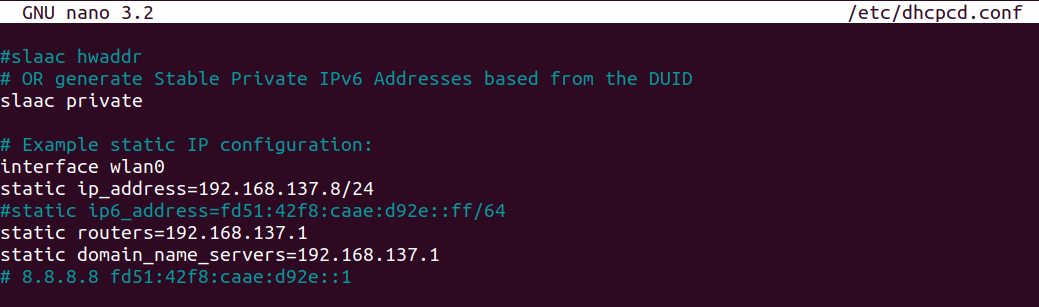
\includegraphics[width=0.9\textwidth]{graphics/dhcpcd.png}
   	\caption{File: dhcpcd.conf} 	
   	\label{pic: dhcpcd}
   \end{figure} 
\item Um Openhabian weiterhin mit Konsole zu erreichen müssen sich die Verschiedenen Geräten, Notebook und Raspi im gleichen IP-Adressraum befinden, eine Änderung kann mittels Adapteroptionen, Eigenschaften Internetprotokoll IPV4, folgende Adresse vergeben, durchgeführt werden.

\item Um Konfigurationen mit Visual Studio Code zu Bearbeiten wird der Ordner openHab-conf in Netzlaufwerk vom Notebook verbunden. Eingabe Ordner: '\textbackslash \textbackslash 192.168.137.8 \textbackslash openHAB-conf' verbinden, mit andern Anmeldedaten anmelden, Username:'openhabian', Passwort: 'openhabian' wählen.

\item In Visual Studio Code Addon 'Openhab' istallieren ,Ordner öffnen openHab-conf wählen. In Einstellungen, Erweiterungen, OpenHab Configuration, Host in 'settings.json' bearbeiten wählen. \\
\colorbox{lightgray}{openhab.host: '192.168.137.8',
	'git.autofetch': true} eingeben. File ist in der Projekt Dokumentation vorhanden. Anschliessend ist ein Neustart von Visual Studio Code erforderlich.
   
   
 \end{enumerate}
\subsection{Openhab Configurieren}

\begin{enumerate}
	\item Openhab Bindings (Schnittstellen) einrichten in Visual Studio Code. In der Ordnerstruktur wird der Ordner 'services' geöffnet und das File 'addons.cfg' bearbeitet. 'binding =' wird ein Kommentiert, das Binding 'mqtt' wird hinzugefügt. Ebenso wird 'misc' ein Kommentiert und 'mqttbroker, openhabcloud' hinzu gefügt gemäss Abbildung \ref{pic: addons.cfg}, anschliessend ist ein Reboot des Raspis notwendig.  
	   \begin{figure}[H]
		\centering
		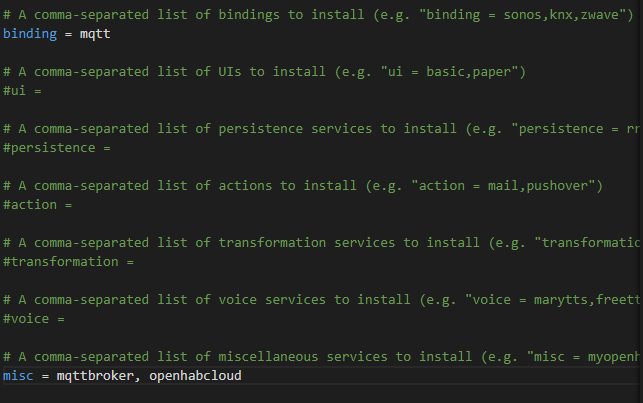
\includegraphics[width=0.9\textwidth]{graphics/addpnscfg.PNG}
		\caption{File: addons.cfg} 	
		\label{pic: addons.cfg}
	\end{figure} 
\item Openhab mit Things (Geräten) verbinden. Things werden im Webinterface hinzugefügt Openhab ist unter URL <IP-Adresse>:8080 erreichbar. Button Paper UI wählen, in der Inbox befindet sich der MQTT Broker, welcher mit einem Click auf den Bestätigungsbutton hinzugefügt wird. 
\item Mit dem Menüpunkt 'Configuration', 'Thing' ist der MQTT Broker sichtbar, mit den blauen add Button werden weitere MQTT-Things hinzugefügt, 'ADD MANUALLY', 'Generic MQTT Thing' wählen, Parameter gemäss Abbildung \ref{pic: Configure MQTT-Thing}  wählen. Dieser Vorgang wird für jedes Bord durchgeführt ein Bord wird als Gerät also als Thing bezeichnet.
	   \begin{figure}[H]
	\centering
	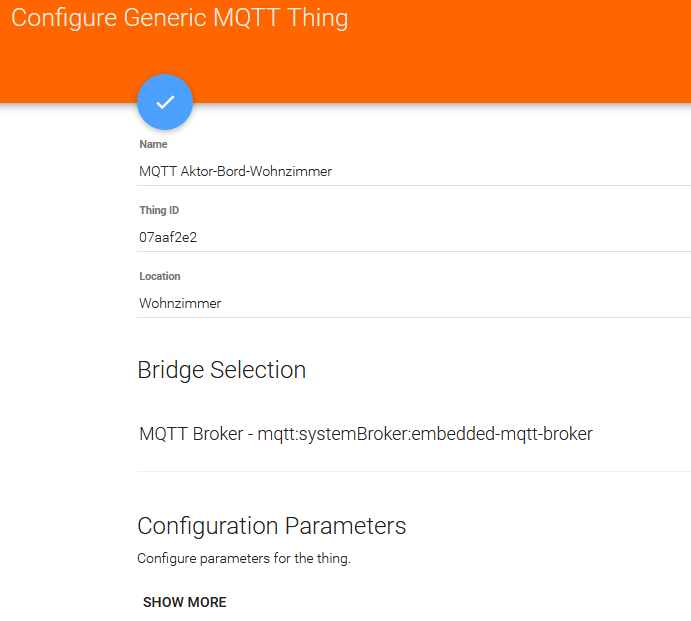
\includegraphics[width=0.75\textwidth]{graphics/MQTT-Thing.PNG}
	\caption{Configure MQTT-Thing} 	
	\label{pic: Configure MQTT-Thing}
\end{figure} 
\item In 'Configuration', 'Thing' ist das nun erstellte Gerät aufgetaucht, dies wählen und Button 'Channels add' wählen, Channel type 'On/OFF Switch' eingeben, Channel id beliebig eingeben, darf keine Leerschläge enthalten, Entsprechende MQTT Configurationen eingeben, Topic siehe Tabelle \ref{tab: MQTT-Topics Aktor}. Für jede Funktion welche in einem Thing (Gerät) enthalten sind, sprich pro MQTT-Topic wird ein Channel gemäss Abbildung \ref{pic: Configure Channel} erstellt.
   \begin{figure}[H]
	\centering
	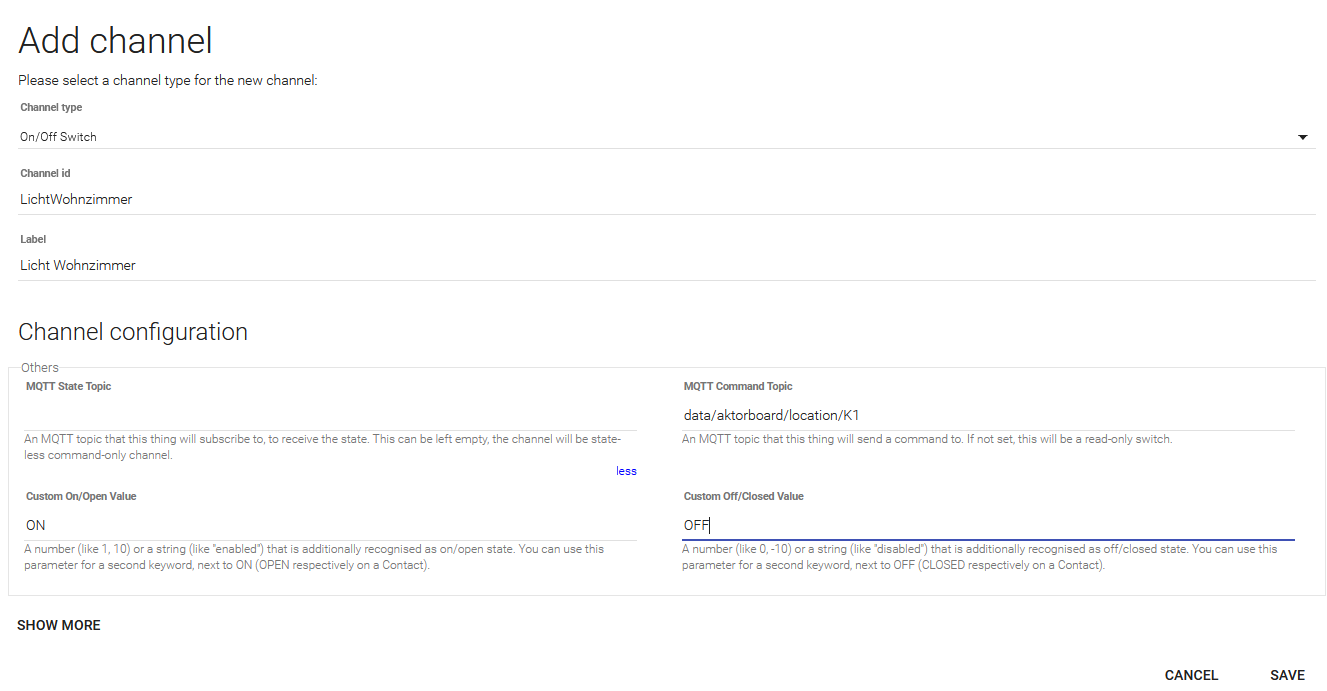
\includegraphics[width=\textwidth]{graphics/Channel.PNG}
	\caption{Configure Channel} 	
	\label{pic: Configure Channel}
\end{figure} 
\item In Visual Studio Code in Ordner 'items' neue Datei erstellen mit Endung .items und öffnen, wird nun das Addon Openhab geöffnet sind zwei Things ersichtlich. Im Tropdown Menü ist das zuvor erstellte item 'Licht Wohnzimmer' ersichtlich und kann in .items Datei importiert werden.
\item Weitere Dateien werden angelegt und Configuriert. Für die Benutzeroberfläche wird im Ordner 'Sitemaps' eine Datei mit Endung .sitemap angelegt ebenso wird für alle Automatischen Vorgängen im Ordner 'rules' eine Datei mit Endung .rules angelegt. Informationen um Items, Rules, oder Sitmaps zu Initialisieren sind unter Dokumentation \cite{noauthor_introduction_nodate} vorhanden.
\item	Fils aus der Projekt-Dokumentation können übernommen werden, dabei muss der Channel Link und Item Bezeichnungen angepasst werden.
\end{enumerate}	